\subsection{Effektives Alphabet}
\label{section:effalphabet}
Sowohl \currentauthor{Hermann Foot} die Laufzeit als auch der Speicherverbrauch einiger der im Framework enthaltenen Algorithmen sind abhängig von der Alphabetgröße des gegebenen Strings. Da das Alphabet allerdings oft mehr Zeichen umfasst als tatsächlich im String vorkommen, kann es sinnvoll sein das vorliegende Alphabet auf die ausschließlich genutzten Zeichen zu reduzieren. Ein solches Alphabet nennen wir effektives Alphabet.\par
\begin{definition}[Effektives Alphabet]
	\label{def:effective_alphabet}
	Sei \(\effective : \Sigma \cup \{\$\} \rightarrow \{0, \ldots, |\Sigma|\}\) eine bijektive Funktion\footnote{\label{differs_from_paper}An dieser Stelle weicht die formale Definition bewusst von der in der zugehörigen Publikation \cite{saca:2} ab, um Definitionslücken für erweiterte Strings zu vermeiden.}, sodass
	\begin{enumerate}
		\item \(\effective(\$) = 0\) \quad und damit \(\forall c \in \Sigma : \effective(\$) < \effective(c)\) und
		\item \(\forall c_1, c_2 \in \Sigma : c_1 < c_2 \Rightarrow \effective(c_1) < \effective(c_2)\).
	\end{enumerate}
\end{definition}
Ziel ist es also eine Abbildung $\effective$ zu konstruieren, die jedes Zeichen in T auf einen Wert im Intervall $[0,|\Sigma|]$ abbildet und dabei die lexikographische Ordnung der Zeichen beibehält, wobei $|\Sigma|$ der tatsächlichen Anzahl vorkommender, unterschiedlicher Zeichen in T entspricht und $\effective(\$)=0$.\\

\begin{figure}[h]
\centering
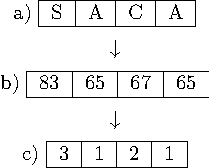
\includegraphics[scale=1]{kapitel/komponenten/techniken/bilder/effExample.pdf}
\caption{Beispiel für ein effektives Alphabet: a) zeigt den Eingabestring b) zeigt die entsprechenden ASCII-Werte c) zeigt die entsprechende effektive Darstellung.}
\end{figure}
Innerhalb unseres Frameworks wird das effektive Alphabet mittels des Objekts \mintinline{cpp}{alphabet} realisiert. Dieses nimmt dazu einen \mintinline{cpp}{string_span} entgegen, merkt sich welche Zeichen darin vorkommen und überschreibt schließlich die Eingabe mit den jeweiligen effektiven Werten. \\
Das Framework bestimmt für jede Eingabe automatisch das effektive Alphabet, welches dann an die Algorithmen übergeben wird. 
